\documentclass{article} % For LaTeX2e
\usepackage{nips13submit_e,times}
\usepackage{hyperref}
\usepackage{url}
\usepackage{graphicx} 
\usepackage[caption=false,font=footnotesize]{subfig}
\renewcommand{\figurename}{\bf Figure}
%\documentstyle[nips13submit_09,times,art10]{article} % For LaTeX 2.09


\title{Biometric in Motion: Identification Using Acceleration Data}


\author{
Zexi Mao\\
\texttt{zexim@andrew.cmu.edu} \\
\And
Siqi Tan \\
\texttt{siqitan@andrew.cmu.edu} \\
\AND
Yuchen Wu\\
\texttt{yuchenw@cs.cmu.edu} \\
\And
Yimeng Zhang \\
\texttt{yimengzh@cmu.edu} \\
}

% The \author macro works with any number of authors. There are two commands
% used to separate the names and addresses of multiple authors: \And and \AND.
%
% Using \And between authors leaves it to \LaTeX{} to determine where to break
% the lines. Using \AND forces a linebreak at that point. So, if \LaTeX{}
% puts 3 of 4 authors names on the first line, and the last on the second
% line, try using \AND instead of \And before the third author name.

\newcommand{\fix}{\marginpar{FIX}}
\newcommand{\new}{\marginpar{NEW}}

\nipsfinalcopy % Uncomment for camera-ready version

\begin{document}


\maketitle

\begin{abstract}
As cellphones and other smart devices are more closer to our daily life than ever, we are curious to know how the data gathered by sensors on the devices, especially identification via accelerometers, impacts our lives. In this project we try to answer this question with the tools machine learning provides. We will first study how to implement such biometric technique by retrieving useful identification information from raw accelerometer data. And then we will show how such technique impacts our lives.
\end{abstract}

\section{Introduction}



\subsection{Motivation}

Ubiquitous computing had never been so close to us as our phones become more powerful and smarter today. Sensors equipped in our cellphones like GPS, gyroscope, accelerometer and even barometer collect data from the surrounding environment and from ourselves. This information collected from our cellphones and other mobile devices can boost many more applications than just adjusting the brightness and rotating the screen. Google uses the GPS data from our phones to provide real-time traffic conditions. Apps can track how well you sleep by just putting your phone beside you on bed. Indoor localization takes advantage of wireless fingerprint, sound from microphone, footsteps from accelerometer and even colours from the camera to tell you where you are when GPS signal is weak inside buildings. More fancy applications far beyond the original purposes of these sensors are on the way. How to retrieve more information from the raw sensor data is one of the hot and promising topics today.

Accelerometer is one of the most interesting sensors in our cellphone which records the acceleration data in 3D. Posture of the phone, gestures and footsteps of the user, and even the user's sleeping condition can be measured by the accelerometer.

In this project, we are trying to develop a novel usage of the accelerometer: biometric identification. In other words, can we identify the user by only looking into how he/she moves? We believe that everyone has his/her own unique pattern of movement. If this assumption is true, we can identify the person when we match the current data from the accelerometer to the historical data we have learned.

To achieve this, we adopt the already available accelerometer dataset gathered by Kaggle. By simply looking into the raw dataset, we can tell not only noise stands between us and our goal, quantity and quality of the raw data also make it harder and more necessary to refine the data before we apply any powerful classifier on it. Our first effect will be on preprocessing data. Then we will adopt several useful technique learned from machine learning to build a classifier for identification. With this preliminary approach, we will further revise and refine both the preprocessor and classifier. Hopefully we will finally achieve a pretty well identification technique in this iterative way. 

If possible, we will evaluate our technique not by testing it on the Kaggle dataset, we will also develop apps for our smart phones to collect real time data for learning and evaluation. We hope this approach will give us the clue of how to protect our id privacy.

We will learn a few things from this project besides a better understanding of machine learning itself if our machine learning algorithms finally identify users. First, the assumption about pattern of movement could be true. Second, applications such as anti-theft, health monitoring and emergency detection that adopt this novel identification technique will be available in the near future. Third, we will be able to know how much data from the accelerometer is sufficient to cause the leak of one's identity, which can trigger a serious privacy issue.


\subsection{Related Work}

A human being’s walking gait can reflect the walker’s physical characteristics and psychological state, and therefore the features of gait can be employed for individual recognition. The use of accelerometer data for biometric identification is relatively new but has been increasingly explored in recent years. Existing methods for gait recognition have shown good performance.
 
Gafurov et al. \cite{Gafurov:AIAT2007} attach multiple sensors to a subject at different body parts. Xu et al. \cite{Xu:ICB2012} developed an Android App to collect gait acceleration data. With a reasonably sized dataset, by matching gait patterns across different paces, they show preliminary results indicating that not only can smart phones be used to identify a person based on their normal gait but also that there is potential to match gait patterns across different speeds.

Tao et al.\cite{Tao:ToPAMI2007} focus on the representation and pre-processing of appearance-based models for human gait sequences. Two major novel representation models are presented, namely, Gabor gait and tensor gait. Experiments show that the new algorithms achieve better recognition rates than previous algorithms.

Pan et al. \cite{Pan:EL2009} proposed algorithm based on signature points, instead of the whole gait signal. They consider acceleration-based gait recognition insensitive to changes of lighting conditions and viewpoint. Their algorithm firstly extracts signature points from gait acceleration signals, and then identifies the gait pattern using a signature point-based voting scheme. The experimental results shows the accelerometer-based gait biometrics is promising. 

Kwapisz et al.\cite{Kwapisz:BTAS2009} collect some data and also perform identification experiments . Based on the 600 raw accelerometer readings, they generated 43 features, which are variations of 6 basic features including average acceleration value, standard deviation, time between peaks and so on. They applied two classification techniques decision trees neural networks to classify and the identification performance turned out to be fairly good.



\section{Methodology}
In this section, we describe the methods we have used to pre-process the raw data and classify the refined data. This is not necessarily the final version of our approach. 

\subsection{The raw data}
The data set acquired from Kaggle consists of 3 parts: a training dataset, a testing dataset and a question set. Each single sample in the training and testing dataset contains a time stamp in milliseconds, acceleration measurements in 3 dimensions, and an associated DeviceId.  There is an Android application published on Google Play for such data collection. This application runs in background while reporting accelerometer data and the corresponding device id to a central server. 

In the training dataset, there are 30 million samples, which are collected from 387 different devices as labeled. In the testing data set, there are also 30 million samples, but without DeviceId. These samples are demarcated into 90,000 sequences, each with a SequenceId. In the question set, for each SequenceId, there's a proposed DeviceId.

The challenge on Kaggle is to tell whether each sequence's proposed DeviceId is the sequence's real DeviceId. For each sequence, we're required to give a belief, in real number, about the credibility of the proposed DeviceId. Therefore, 

 \emph{For our study, we aim at a more general version of the problem of classification, which is telling the correct DeviceId for any given sequence of sample.}

\subsection{Refinement}
The raw dateset has already been prepared preliminarily by Kaggle. First, the devices with fewer than 6000 samples are removed ahead. Second, sequences of samples during periods of rest exceeding 10 seconds are eliminated as well. 

\begin{figure}
    \hspace{-0.5cm}
    \begin{minipage}[t]{0.02\textwidth}~
    \end{minipage}
    \begin{minipage}[t]{0.47\textwidth}
    \centering
    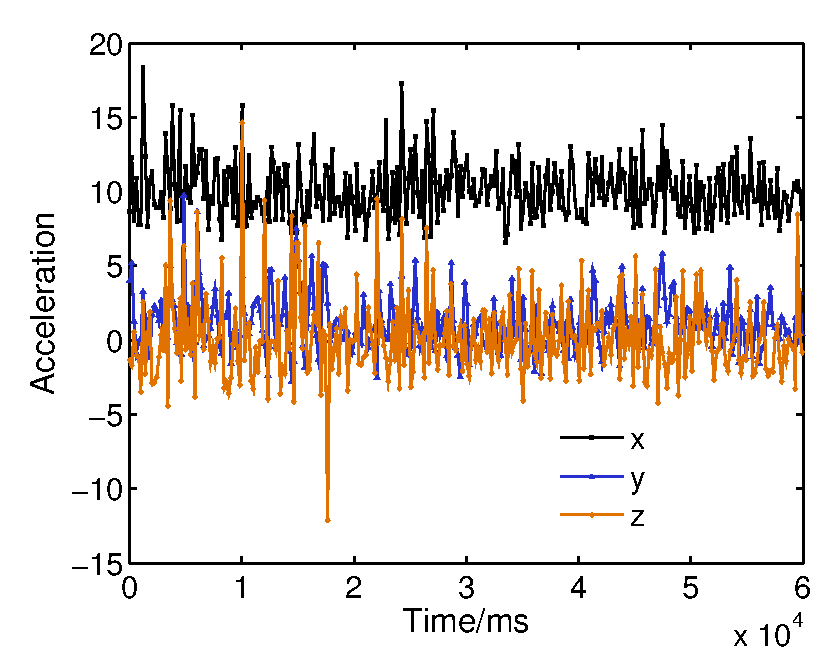
\includegraphics[height=40mm]{fig/good_raw.eps}
    \caption{A good trace of raw data. Data is almost uniformly distributed along time. }
    \label{fig:good_raw}
    \end{minipage}
    \begin{minipage}[t]{0.02\textwidth}~
    \end{minipage}
    \begin{minipage}[t]{0.47\textwidth}
    \centering
    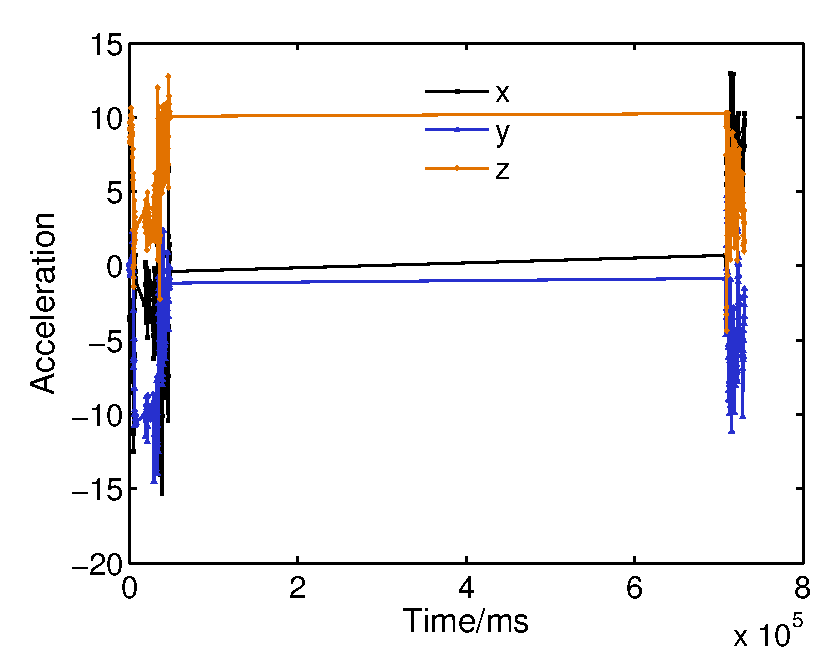
\includegraphics[height=40mm]{fig/bad_raw.eps}\\
    \caption{A bad trace of raw data. This piece essentially contains information about 2 separate activities that are far apart in time.}
    \label{fig:bad_raw}
    \end{minipage}
    \begin{minipage}[t]{0.02\textwidth}~
    \end{minipage}%   
 \end{figure}


However, the dataset is still far from beautiful.

First, accelerometers have various sampling rates. A large interval between two samples may lead to much information loss between the two sample points. Furthermore, the acceleration on each dimension changes rapidly in such low sample rate. The high variance of sampling interval within one device's trace even makes it harder to retrieve features.

Second, according to the nature of Android system and the low privilege of an application, sometimes the app cannot access the accelerometer, sometimes the app itself is swapped out or killed by the operating system. Thus, a great part of the sample data is not well distributed over time.

Figures \ref{fig:good_raw} and \ref{fig:bad_raw} show the two segments of untouched raw data. 

To overcome the two challenges above. We propose our three phase refinement: splitting, smoothing and re-sampling.

The idea of splitting is very simple. For the first step of splitting, we scan a sequence of data from a identical device in chronological order. Once the interval between our current sample point and the previous one is greater than a threshold $T_\mathrm{split}$, the samples scanned before are grouped into one sub-sequence. This process continues until all the data from each identical device is split completely. Then we go to the step two of splitting. In this step, if any sub-sequence is shorter than a threshold $T_\mathrm{short}$, we simply eliminate it as we believe that a too short sequence brings more noise than useful information. If, unfortunately, all the data from a particular device is abandoned, it left us no choice but keeping the longest among its all sub-sequences.

The next phase is to make the sequence smoother, which hopefully could reduce the level of noise. To this end, interpolation is the idea that comes to us so far. We simply adopt cubic spline as our interpolating function. Thus, we transform a sequence of sample points into a continuous curve. Some missing pieces of data are ``reproduced'' in this way. This phase makes it easier for feature retrieval as we can now get the data at any time point. We should notice that noise is not necessarily reduced well in this manner. The curve we get contains almost the whole noise from the original data as it is with respect to every single data point from the raw data. We believe a better smoothing function will help while we are still looking for such one.

The third phase benefits from the smoothing phase as it is quite easy to re-sample data point from a smooth curve. We set a parameter, $\tau_\mathrm{resample}$, to be the re-sampling time interval. With this interval, a new sequence of data is generated from on the (interpolated) original data trace.

After the three phases, the refined data trace is produced from the raw data. Next, we will propose the way we select features from such refined trace.

\subsection{Feature extraction}
Feature selection as well as extraction is the most important part of the entire classification process. A great feature should pinpoint reveal the underlying differences between the users (also known as DeviceId in this project). In this section, we describe how to extract features from the data.
	
\subsubsection{Frequency domain features}
The only assumption we made so far in this research project is that a human being moves in his/her own characteristic pattern. This pattern could be a sequence of outstanding events, or it could be some repeated, characteristic events as well. Noticing that accelerometer records data with unpredictable length and quality, we cannot assume that the complete sequence of events could be well recorded. Thus, our hope rests on the latter one. 

It is customary to use frequency analysis for repeated events. In our approach so far, simple Fast Fourier Transformation is adopted. The basic idea is just making FFT on the refined data sequence we talked about in previous section.

A better idea is to make windowed FFT on them. The reason is, as each of the sequence has different length, if we make full FFT on each sequence, the frequency components produced by FFT have different meanings on different lengths of FFT. For example, we make full FFT on two sequence with length 17 and 29 respectively, the resultant points are not matched in the frequency domain. The results will be hard to be interpreted and compared. To this end, we make the transformation in a given window size, $w_\mathrm{fft}$. Thus, multiple transformations are performed in a sliding window manner. We can average each corresponding points from different transformations, as they are matched in the frequency domain. 

However, another concern arises. If we make one windowed FFT on a pretty long sequence, some information is erased by the sliding window averaging. This is true if we believe that a longer sequence could contain more information than a shorter one.

To this end, we prefer to perform partitioning on long sequences before doing windowed FFT. There are two thresholds in the partitioning process. One is the lower bound of number of generated sub-sequences, $k_\mathrm{\#seq}$, the other is the upper bound of the maximum length among all the generated sub-sequences, $l_\mathrm{maxL}$. The procedure of partitioning goes as follows. The input sequence is halved into two sub-sequences until either of the following conditions satisfied: a) the number of sub-sequences is greater than $k_\mathrm{\#seq}$; b) all the sub-sequences are shorter than $l_\mathrm{maxL}$. In this manner, on the one hand, we make more sequences from one device, hopefully keeping more information about the device's diverse patterns. On the other hand, we use the second threshold to make the sequences not too short, so that they contain reliable information about patterns of the device.

So far, the results of FFT is the extracted features as we shown above. As there are three dimensions, and the independent values of FFT with window size $w_{fft}$ is $1/2w_{fft}$, we build a feature space with $3/2w_{fft}$ dimensions.

\subsubsection{Time domain features}
As the mobile devices people use are increasingly diverse, the characteristics of different devices offer us a set of very distinguishing features for recognizing users. One of these characteristics is the sampling frequencies of devices.

As we observed from the timestamps of training data of each device, the sampling frequencies of devices has a range of approximately 10-250ms. Thus, we used the histogram of differences of timestamps in each sample as the time domain features.

\subsubsection{Accelerometer reading features}
Apart from the sampling times of devices, we found another set of features with potential ability of distinguishing devices, which is the accelerometer readings.

During observation of data, we found that each kind of device can only provide certain discrete values, this may be due to the accuracy limitation of accelerometers. Thus, the set of accelerometer readings a device can provide is also treated as a set of features.

\subsection{Classification}
This is the ongoing part of out work. The basic idea is to leverage various kinds of classifiers and optimize their parameter for more accurate results.

We start from some naive classifiers. The performance of K-Nearest-Neighbor depends on the number of K and the definition of distance function. This classifier leads us to a baseline result. Then we move on to popular classifier such as support vector machine. Optimizing SVM via kernel and parameter selection will be discussed in next section.

\section{Implementation and Evaluation}
In this section we show how our approach performs. We will also manipulate and justify the selection of parameters of both reprocessing and classifiers.

\subsection{Parameter selection}
In this subsection we discuss how to determine the parameters and thresholds we defined in the previous sections.

$T_{splite}$ is set to be 10 second in consistent with the preprocessing setting done by Kaggle. It is pointless to set the threshold above 10 seconds as those sequence shorter than 10 seconds have already been eliminated. We keep this threshold as large as possible to generate longer continues sequences. $T_{short}$ is set as 4.8 seconds for training set and 3.2 seconds for test set based on empirical study. 

We let $\tau_{resample}$ be 200 millisecond. This value is chosen based our statistic result of the distribution of the original data. Any value near 200 ms is a reasonable choice because most of the intervals lie in this range. Choosing a value deviating from 200 ms could misinterpret the data. (put a figure here for CDF of interval?)

The window size of FFT, $w_{fft}$, is 64 sample points, which means a window with length 12.8 seconds. We chose this value to balance the details of data and dimensions of feature space. 

$k_{\#seq}$ and  $l_{maxL}$ are more flexible as the result is less sensitive on these values.

\subsection{Optimizing classifier}
This is the To Be Done part.

\subsection{Results}

According to the rules of this compitition, classification results are judged on area under the ROC curve. Three main kinds of classifiers we have used are k-nearest neighbors, SVM with Gaussian kernel and $L_2$-regularized logistic regression. The results comparing with the compitition baseline, using k-NN of the mean values of the values in 3 dimension, is shown in Table 1.

\begin{table}[!ht]
\caption{Testing results of four methods}
	\begin{center}
		\begin{tabular}{ c | c  c  c  c }
			\hline
			 Methods & k-NN Mean & k-NN FFT & SVM & Regression \\
			 \hline
			 AUC & 0.50277 & 0.58590 & 0.79801 & 0.89729 \\
			 \hline
		\end{tabular}
	\end{center}
\end{table}

\section*{Appendix}

Our plan for future goes here.


\bibliographystyle{IEEEtranS}
\bibliography{references}



\end{document}
